\begin{figure}[h]
    \centering
    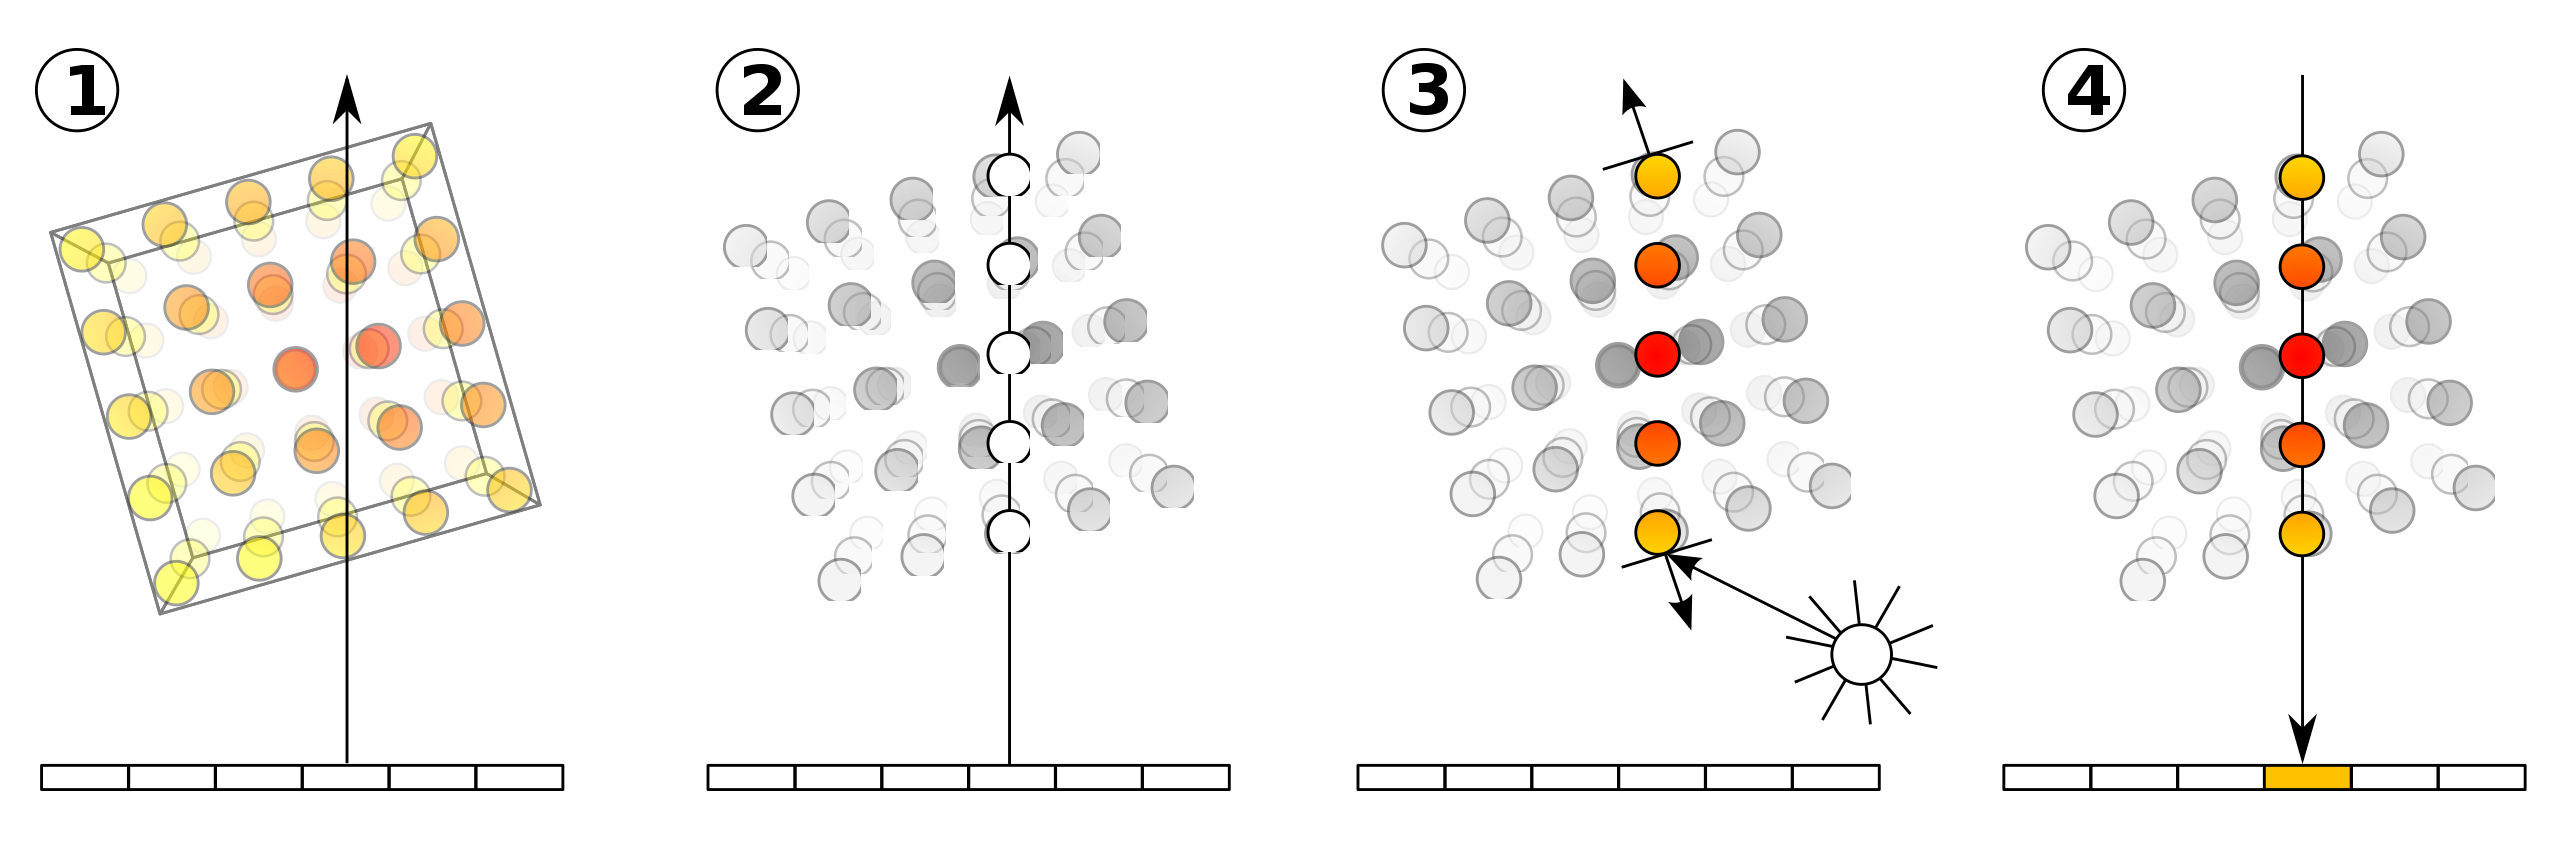
\includegraphics[width=1.0\textwidth]{figures/volume-rendering.png}
    \caption{The four basic steps of volume rendering \cite{wiki:Volume_ray_casting}. 1) A ray is cast from the image plane into the volume. 2) Points in the volume are sampled. 3) The points are shaded based on their $RGB\alpha$-value and the illumination-value gradients in relationship with the local light source. 4) The final pixel color is obtained by compositing all the shaded samples along the ray.}
    \label{fig:volume-rendering}
\end{figure}